% vim: ts=8 sts=8 sw=4 et tw=75
\chapter{算法实验}
\label{chap:experiments_with_algorithms}
\marginpar{153}

一般而言, 理解事物如何工作的最好方式就是自己动手做一些小实验, 算法学习
就是一个典型的例子: 编写实际代码有助于弄清楚那些容易被伪码掩盖的问题.
不仅如此, 最终得到的程序是运行的, 通过观察运行结果, 就可以知道算法的
的正确性, 而这是伪码所无法办到的.

Awk 很适合做这种测试工作. 如果某个程序使用 awk 编写, 那我们就可以把精力
集中在算法上, 而不是语言本身. 如果某个算法最终要应用到某个大型程序中,
那么先让算法能够单独地运行起来可能会更有效率. 当需要为某个算法进行调试,
测试与性能评价时, 通常需要构造一些脚手架程序, 在这一方面, awk 是一款
优秀的脚手架构造工具, 它并不管算法本身是用什么语言实现的.

这一章讨论算法实验. 前半章描述三种排序算法, 这三种算法常常是算法课首
先要介绍的内容, 我们将使用 awk 程序对这些算法进行测试, 性能度量和
刻画. 后半章展示几种拓扑排序算法, 实现 Unix 的文件更新实用程序
\texttt{make}.

\section{排序}
\label{sec:sorting}

这一小节讨论三种著名并且很有用的算法: 插入排序, 快速排序, 以及堆排序.
插入排序非常简单, 但是只有在元素很少的情况下, 效率才足够高; 快速排序
是最好的通用排序算法之一; 堆排序可以保证即使在最坏的情况下, 也可以拥有
较高的效率. 我们对每一种算法都进行介绍, 并加以实现, 然后再用测试例程
对它们进行测试, 最后评价性能.

\subsection{插入排序}
\label{subsec:insertion_sort}
\cterm{基本概念}. 插入排序的过程类似于给一堆卡片排序: 每次从卡片堆里
拿出一张, 把它插入到合适的位置.\footnote{原文为 Insertion sort is similar
    to the method of sorting a sequence of cards by picking up the cards
    one at a time and inserting each card into its proper position in the
hand}
\marginpar{154}
\cterm{实现}. 下面的代码使用插入排序对数组 \texttt{A[1]}, ...,
\texttt{A[n]} 进行升序排列. 第一个动作把输入数据读取到一个数组中,
\texttt{END} 动作调用函数 \texttt{isort} 对数组进行排序, 最后输出排序
结果:
\begin{awkcode}
    # insertion sort 
        { A[NR] = $0 }
    END { isort(A, NR)
          for (i = 1; i <= NR; i++)
              print A[i]
        }

    # isort - sort A[1..n] by insertion
    function isort(A, n,    i, j, t) {
        for (i = 2; i <= n; i++)
            for (j = i; j > 1 && A[j-1] > A[j]; j--) {
                # swap A[j-1] and A[j]
                t = A[j-1]; A[j-1] = A[j]; A[j] = t
            }
    }
\end{awkcode}
\texttt{isort} 函数内的外层循环在每次迭代开始时, 数组\texttt{A} 的元素
\texttt{1} 至 元素 \textit{i}\texttt{-1} 处于有序状态. 内层循环每次迭代
都把当前处于第 \textit{i} 个位置上的元素向前移动, 跳过所有比它大的元素. 
当外层循环结束时, 所有的 \textit{n} 个元素都处于有序状态.

数值或字符串都可以用这个程序进行排序. 但是当输入数据同时含有数值与字符
串时, 就要小心一点 --- 由于强制类型转换, 比较结果可能会让你感到惊讶.

如果数组 \texttt{A} 含有以下 8 个整数:
\begin{file}
    8 1 6 3 5 2 4 7
\end{file}
那么排序的过程如下所示:
\begin{file}
    8|1 6 3 5 2 4 7
    1 8|6 3 5 2 4 7
    1 6 8|3 5 2 4 7
    1 3 6 8|5 2 4 7
    1 3 5 6 8|2 4 7
    1 2 3 5 6 8|4 7
    1 2 3 4 5 6 8|7
    1 2 3 4 5 6 7 8|
\end{file}
竖线符把数组的已排序部分和未排序部分分开.

\cterm{测试}. 应该如何测试 \texttt{isort}? 我们可以每次输入一点数据,
并查看排序结果, 当然, 这样做并没有错, 可是对于任意规模的程序来说, 
这种方法不能做到详尽的测试. 第二种方案是自动生成大量的随机数集合, 
把这些集合作为 \texttt{isort} 的输入数据. 这的确是一个不错的办法,
但是还可以做得更好: 为了测试程序的薄弱环节, 我们还需要构造一些特殊
的测试用例, 测试边界与异常情况.
\marginpar{155} 对排序来说, 典型的边界或异常情况包括:
\begin{pattern}
\indent\indent 序列长度为 0 \par
\indent\indent 序列长度为 1 \par
\indent\indent 序列包含 \textit{n} 个随机数 \par
\indent\indent 序列包含 \textit{n} 个已排序的数 \par
\indent\indent 序列包含 \textit{n} 个逆序排列的数 \par
\indent\indent 序列包含 \textit{n} 个相同的数
\end{pattern}

本章的目标之一是展示如何使用 awk 来帮助测试和评价程序. 为了说明, 我们现在
要对排序例程的测试与结果评价进行自动化.

主要有两种办法来实现测试与评价过程的自动化, 每一种都有它各自的优点. 第一 
种称为 ``批处理模式'': write a program to execute a pre-planned set of
tests, exercising the sort function as suggested above.\footnote{TODO}
下面的程序可以生成测试数据并检查测试结果. 除了 \texttt{isort}, 还有其他
几个函数, 它们用来生成不同类型的数组, 以及检查排序后的数组是否是有序的.
\begin{awkcode}
    # batch test of sorting routines

    BEGIN {
        print "    0 elements"
        isort(A, 0); check(A, 0)    
        print "    1 element"
        genid(A, 1); isort(A, 1); check(A, 1)
        
        n = 10
        print "    " n " random integers"
        genrand(A, n); isort(A, n); check(A, n)
        
        print "    " n " sorted integers"
        gensort(A, n); isort(A, n); check(A, n)
        
        print "    " n " reverse-sorted integers"
        genrev(A, n); isort(A, n); check(A, n)
        
        print "    " n " identical integers"
        genid(A, n); isort(A, n); check(A, n)
    }

    function isort(A,n,     i,j,t) {
        for (i = 2; i <= n; i++)
            for (j = i; j > 1 && A[j-1] > A[j]; j--) {
                # swap A[j-1] and A[j]
                t = A[j-1]; A[j-1] = A[j]; A[j] = t
            }
    }

\end{awkcode}
\marginpar{156}
\begin{awkcode}
    # test-generation and sorting routines...

    function check(A,n,   i) {
        for (i = 1; i < n; i++)
            if (A[i] > A[i+1])
                printf("array is not sorted, element %d\n", i)
    }

    function genrand(A,n,  i) { # put n random integers in A
        for (i = 1; i <= n; i++)
            A[i] = int(n*rand())
    }

    function gensort(A,n,  i) { # put n sorted integers in A
        for (i = 1; i <= n; i++)
            A[i] = i
    }

    function genrev(A,n,  i) {  # put n reverse-sorted integers
        for (i = 1; i <= n; i++)  # in A
            A[i] = n+1-i
    }

    function genid(A,n,  i) {   # put n identical integers in A
        for (i = 1; i <= n; i++)
            A[i] = 1
    }
\end{awkcode}

第二种方法相对来说没那么方便, 但很适合用 awk 来处理. 基本思想是构建一个
构架程序, 利用该框架可以很容易以交互性的方式来完成测试. 交互式方案是
批处理模式的一个很好的补充, 特别是当待测试的算法没有排序那么容易理解
时. 交互式处理模式在调试程序时也很方便.

特别地, 我们将要设计的程序, 在效果上等价于一个专门用于构造测试数据与操作
的微型语言, 因为语言并不需要做太多的工作, 也不必处理大量用户的情况,
所以不用设计得多么复杂. 如果必要的话, 我们甚至可以丢掉写了一半的代码,
重新开始. Our language provides for automatic generation of an array, and,
looking ahead to the rest of this chapter, for naming the sort to be
exercised.\footnote{TODO} 我们省略了排序和数据生成子程序, 它们和前一个
示例相同.

程序的基本组织是一系列的正则表达式, 它们负责扫描输入数据, 判断数据类型
和使用的排序算法. 如果某个输入数据不与任何一个模式相匹配, 程序就会输出
一条错误消息, 并演示正确的使用方法. 如果仅仅说明输入数据有错, 可能没
多大帮助.

\marginpar{157}
\begin{awkcode}
    # interactive test framework for sort routines

    /^[0-9]+.*rand/ { n = $1; genrand(A, n); dump(A, n); next }
    /^[0-9]+.*id/   { n = $1; genid(A, n); dump(A, n); next }
    /^[0-9]+.*sort/ { n = $1; gensort(A, n); dump(A, n); next }
    /^[0-9]+.*rev/  { n = $1; genrev(A, n); dump(A, n); next }
    /^data/ {   # use data right from this line
            for (i = 2; i <= NF; i++)
                    A[i-1] = $i
            n = NF - 1
            next
    }
    /q.*sort/ { qsort(A, 1, n); check(A, n); dump(A, n); next }
    /h.*sort/ { hsort(A, n); check(A, n); dump(A, n); next }
    /i.*sort/ { isort(A, n); check(A, n); dump(A, n); next }
    /./  { print "data ... | N [rand|id|sort|rev]; [qhi]sort" }

    function dump(A, n) {    # print A[1]..A[n]
            for (i = 1; i <= n; i++)
                    printf(" %s", A[i])
            printf("\n")
    }

    # test-generation and sorting routines ...
    ...
\end{awkcode}
正则表达式提供了一种非常宽松的输入语法: 只要短语和快速排序稍微有点接近,
比如 ``quicksort'', 就选择快速排序算法. 我们也可以直接手工输入数据, 
而不是自动生成, 这个功能允许我们既可以基于文本, 也可以基于数字对算法
进行测试. 为了说明, 上面程序的一个输出是:
\begin{shell}
    10 random 
     9 8 4 6 7 2 4 0 4 0
    isort 
     0 0 2 4 4 4 6 7 8 9
    10 reverse 
     10 9 8 7 6 5 4 3 2 1
    qsort
     1 2 3 4 5 6 7 8 9 10 
    data now is the time for all good men
    hsort
     all for good is men now the time
\end{shell}

\cterm{性能}. \texttt{isort} 所执行的操作次数取决于 \textit{n} 的值,
即待排序的元素个数, 以及它们原来的排列顺序. 插入排序是 \cterm{平方} 级
算法, 也就是说, 在最坏的情况下, 算法的运行时间增长速度与元素个数的平方成
正比. 这意味着如果元素个数变成原来的 2 倍, 那么运行时间将会是原来的
4 倍. 如果待排序元素碰巧就处于一种基本有序的状态, 那么程序的工作量
就会少很多, 于是运行时间将会按照线性增长, 线性增长指的是与元素的个数
成正比.

\marginpar{158}
下面这副图显示了 \texttt{isort} 面对三种类型的数据时的性能变化情况, 
这三种类型分别是: 逆序序列, 随机序列, 以及同一个元素组成的序列. 
我们计算了比较
和交换的次数, 对于一个排序过程来说, 这是两个很客观的指标. 正如你
所看到的那样, 逆序序列拥有最差的性能, 随机序列居中, 而同一元素
序列表现出了最佳的性能. 有序序列的性能再现和同一元素序列非常接近
(在图中没有显示出来). \footnote{TODO}

总得来说, 插入排序适用于元素个数较少的情况, 当元素个数过多时, 该算法
的性能就会快速下降, 除非输入数据基本有序.

通过为每个排序函数添加两个计数器, 我们就可以为上面的图, 以及本章中的
其他图生成所需要的数据. 一个计数器计算比较的次数, 另一个计算交换的次数.
这是带计数功能的 \texttt{isort} 函数:
\begin{awkcode}
    function isort(A,n,     i,j,t) {  # insertion sort
        for (i = 2; i <= n; i++)      # with counters
            for (j = i; j > 1 && ++comp &&
              A[j-1] > A[j] && ++exch; j--) {
                # swap A[j-1] and A[j]
                t = A[j-1]; A[j-1] = A[j]; A[j] = t
            }
    }
\end{awkcode}
计数操作都放在内层 \texttt{for} 循环的条件判断部分完成.由 \verb'&&' 
连接的条件判断, 按照从左到右的顺序进行求值, 直接某一项为假. 表达式
\texttt{++comp} 总是为真 (这里必须使用前缀形式的自增运算符), 于是,
数组中的元素每比较一次, \texttt{comp} 的值就加 1, 递增操作在比较之前
完成. 当且仅当某两个元素被交换时, \texttt{exch} 的值才会加 1.
\marginpar{159}

下面的程序用于组织测试, 以及为坐标图准备数据. 同样, 它的功能相当于一
个微型编程语言, 可以用来指定参数.
\begin{awkcode}
    BEGIN { srand(1111) }
    { print }
    # interactive test framework for sort routines

    /^[0-9]+.*rand/ { n = $1; genrand(A, n); dump(A, n); next }
    /^[0-9]+.*id/   { n = $1; genid(A, n); dump(A, n); next }
    /^[0-9]+.*sort/ { n = $1; gensort(A, n); dump(A, n); next }
    /^[0-9]+.*rev/  { n = $1; genrev(A, n); dump(A, n); next }
    /^data/ {   # use data right from this line
            for (i = 2; i <= NF; i++)
                    A[i-1] = $i
            n = NF - 1
            next
    }
    /q.*sort/ { qsort(A, 1, n); check(A, n); dump(A, n); next }
    /h.*sort/ { hsort(A, n); check(A, n); dump(A, n); next }
    /i.*sort/ { isort(A, n); check(A, n); dump(A, n); next }
    /./  { print "data ... | N [rand|id|sort|rev]; [qhi]sort" }

    function dump(A, n) {    # print A[1]..A[n]
            for (i = 1; i <= n; i++)
                    printf(" %s", A[i])
            printf("\n")
    }

    # test-generation and sorting routines ...

\end{awkcode}
输入数据是由多行组成的序列, 类似于
\begin{shell}
    isort random 0 20 40 60 80 100 
    isort ident 0 20 40 60 80 100
\end{shell}
输出数据的每一行都包括名字, 类型, 大小, 以及每一种大小的数量.\footnote{
    原文为 And the output consist of lines containing the name, type, size,
and counts for each size.}  输出数据被输送给绘图程序 \texttt{grap}, 它
是我们在第 \ref{chap:little_languages} 章讨论的绘图程序的原始版本.

\begin{exercise}
    实际上, 函数 \texttt{check} 并不是一个很强大的测试, 什么样错误会
    使它检测失败? 你会如何改进?
\end{exercise}

\begin{exercise}
    我们的大多数测试都基于整数排序, 面对其他类型的数据时, \texttt{isort}
    的表现会如何? 为了处理更一般的数据, 你会如何改进测试框架程序?
\end{exercise}

\begin{exercise}
    我们默认每一种基本操作都需要相同的时间, 也就是说, 访问一个元素, 比较 
    两个元素的值, 加法, 赋值等操作所消耗的时间是相同的. 对于 awk 程序来说 
    这个假设是否合理? 写一个处理大量数据的程序, 来验证你的想法.
\end{exercise}
\marginpar{160}

\subsection{快速排序}
\label{subsec:quicksort}

\cterm{基本概念}. 快速排序是最高效的通用排序算法之一, 由 C. A. R. Hoare
在六十年代早期提出. 为了对一个元素序列进行排序, 快速排序算法把序列划分成
两个子序列, 然后再递归地对子序列进行排序. 在划分阶段, 算法从序列中选取
一个元素作为划分点, 把剩下的元素分成两组: 小于划分元素的分在一个组中, 
而大于或等于划分元素的分在另一个组中, 然后再对这两组递归调用快速排序.
如果一个序列所含的元素个数小于2, 则可认为它已经是有序的了, 于是算法
什么也不做就返回.

\cterm{实现}. 实现快速排序有多种方式, 这些方式的不同点就在于划分阶段.
我们所选择的实现方式比较容易理解, 虽然不是最快的. 因为算法是递归的,
所以我们会在划分操作作用在子数组 \texttt{A[left]}, \texttt{A[left+1]},
..., \texttt{A[right]} 上时, 对划分进行描述.

首先需要选择一个划分元素: 从范围 \texttt{[left,right]} 中随机选取一个数
\texttt{r} 作为划分点, 任何一个元素都可以作为划分点, 但是如果序列已经具
有了某种程度上的有序, 那么随机选择会工作得更好. 位置 \texttt{r} 上的元素
\texttt{p} 现在成了划分元素. 交换 \texttt{A[left]} 与 \texttt{A[r]},
在划分的过程中, 数组始终把元素 \texttt{p} 放在 \texttt{A[left]}, 
\texttt{A[left]} 的后面是比 \texttt{p} 小的元素, 再接下来是大于或等于
\texttt{p} 的元素, 最后是到目前为止未处理的元素:\footnote{TODO}

下标 \texttt{last} 指向最后一个比 \texttt{p} 小的元素, 下标 \texttt{i}
指向下一个未处理的元素. 初始化时, \texttt{last} 等于 \texttt{left},
\texttt{i} 等于 \texttt{left+1}.

在划分过程的循环中, 我们比较元素 \texttt{A[i]} 与 \texttt{p}. 如果 
\texttt{A[i] >= p}, 只需要递增 \texttt{i} 即可; 如果 \texttt{A[i] < p},
此时需要递增 \texttt{last}, 并交换 \texttt{A[last]} 与 \texttt{A[i]},
最后再递增 \texttt{i}. 按照这种方式, 一旦所有的元素都处理完毕, 我们需要
交换 \texttt{A[left]} 与 \texttt{A[last]}. 到这里, 我们已经完成的一次
划分, 此时的数组看起来就像这样:\footnote{TODO}
\marginpar{161}
现在, 我们对左边的子数组与右边的子组执行同样的操作.

假设我们对下列8个元素进行快速排序:
\begin{file}
    8 1 6 3 5 2 4 7
\end{file}
第一步我们可能选择 4 作为划分元素, 接下来, 划分操作会把数组重新排列成
\begin{file}
    2 1 3|4|5 6 8 7
\end{file}
接下再递归地对子数组 \texttt{2 1 3} 与 \texttt{5 6 8 7} 进行快速排序. 
我们可以用插入排序的测试例程对该算法进行测试.
\begin{awkcode}
    # quicksort

        { A[NR] = $0 }

    END { qsort(A, 1, NR)
          for (i = 1; i <= NR; i++)
              print A[i]
        }

    # qsort - sort A[left..right] by quicksort

    function qsort(A,left,right,   i,last) {
         if (left >= right)  # do nothing if array contains
             return          # less than two elements
         swap(A, left, left + int((right-left+1)*rand()))
         last = left   # A[left] is now partition element
         for (i = left+1; i <= right; i++)
             if (A[i] < A[left])
                 swap(A, ++last, i)
         swap(A, left, last)
         qsort(A, left, last-1)
         qsort(A, last+1, right)
    }

    function swap(A,i,j,   t) {
         t = A[i]; A[i] = A[j]; A[j] = t
    }
\end{awkcode}

\cterm{性能}. \texttt{qsort} 所执行的操作次数取决于数组划分时的均匀程度.
如果数组划分每次都很平均, 那么程序的运行时间与 $n \log n$ 成正比.
\marginpar{162}
于是, 如果数据规模变为原来的两倍, 那么程序的运行时间只会在原来两倍的基础上
再稍微多出一点.

在最坏的情况下, 划分操作的结果会出现其中一个子数组长度为 0 的情况, 比如,
当所有元素都相同时, 就会出现这种情况. 这时候, 快速排序的时间复杂度就
会退化到二次方. 幸运的是, 对于随机数据来说, 不会出现这种极不均匀的划分. 
下面这张图显示了快速排序面对三种类型的输入数据时的性能表现 (在测试插入
排序时, 也用到了这三种类型的数据). 正如你所看到的那样, 对于同元素序列
来说, 操作次数的增长速度要比另外两种类型的增长速度快得多. \footnote{应该 
用矢量图, 而不是从原版中截图 --- 译者注}

\begin{center}
    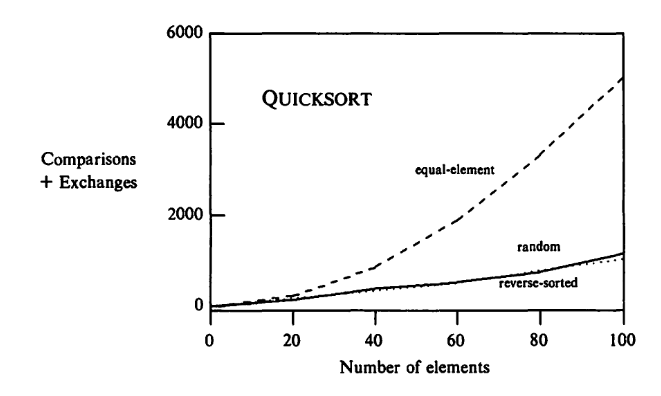
\includegraphics[scale=0.7]{images/quicksort.png}
\end{center}

\begin{exercise}
    为 \texttt{qsort} 添加计数语句, 计算比较操作和交换操作的执行次数.
    你得到的结果是否和我们的类似 ?
\end{exercise}

\begin{exercise}
    记录程序的运行时间, 而不是操作次数. 运行时间的统计图是否和操作次数
    的相同 ? 用大一点的例子作测试, 看看其统计图还是不是一样的.
\end{exercise}

\cterm{基本概念}. \cterm{优先级队列} (\term{priority queue}) 是一种数据
结构, 用于存储和检索元素. 它有两种基本操作: 往队列中插入一个新元素, 以及 
从队列中提取最大的元素. 这表明优先级队列可以用来排序: 首先把所有的元素
插入到队列中, 然后每次抽取一个元素. 因为每次移除的都是最大的元素, 所以 
元素是以降序地方式从队列中抽取出来. 这种排序方法叫作堆排序, 由
J. W. J. Williams 和 R. W. Floyd 在 60 年代早期提出.

\marginpar{163}
堆排序使用一种称为 \cterm{堆} (\term{heap}) 的数据结构来维护优先级队列,
我们可以把堆想像成一棵二叉树, 但是带有两条额外的性质:
\begin{enumerate}
    \item 树是高度平衡的: 叶子结点最多只在两个不同的层次上出现, 另外,
        位于最底层 (距离根结点最远的层次) 的叶子尽量靠左排列;
    \item 树是部分有序的: 每个结点的值大于或等于它的孩子结点.
\end{enumerate}
这是带有 10 个元素的堆:\footnote{TODO}

堆具有两条非常重要的性质. 第一条性质是如果有 \textit{n} 个结点, 那么所
有的从根结点到叶子结点的路径长度都不会大于 $\log_2^n$. 第二条性质是
具有最大值的元素总是在根结点 (这个位置称为 ``堆顶'').

如果我们用一个数组 \texttt{A} 来模拟堆, 那么就不需要构造显式的二叉树.
树中的结点按照宽度优先遍历的顺序出现在数组中, 也就是说, 根结点在 
\texttt{A[1]}, 它的左孩子与右孩子分别在 \texttt{A[2]} 和 \texttt{A[3]}.
总的来说, 如果某个结点在 \texttt{A[}\textit{i}\texttt{]}, 那么它的孩子就
在 \texttt{A[2}\textit{i}\texttt{]} 和 \texttt{A[2}\textit{i}\texttt{+1]},
如果只有一个孩子的话, 那就在 \texttt{A[2}\textit{i}\texttt{]}.
于是, 上面那棵树对应的数组 \texttt{A} 就是:\footnote{TODO}

堆的部分有序性质指的是元素 \texttt{A[}\textit{i}\texttt{]} 大于或等于
它的孩子结点 \texttt{A[2}\textit{i}\texttt{]} 与
\texttt{A[2}\textit{i}\texttt{+1]}, 如果只有一个孩子的话, 就那大于或等于
\texttt{A[2}\textit{i}\texttt{]}. 如果某个数组满足这个条件, 我们就说
这个数组具有 ``堆属性''.

\cterm{实现} (\term{Implementation}). 堆排序由两个阶段组成: 构造堆, 以及 
按顺序从堆中提取元素. 两个阶段都要调用函数 \texttt{heapify(A,i,j)}, 使得
子数组 \texttt{A[i]},\texttt{A[i+1]},...,\texttt{A[j]} 具有堆属性 (假设 
\texttt{A[i+1]},...,\texttt{A[j]} 已经具有了堆属性). \texttt{heapify}
的基本操作是比较 \texttt{A[i]} 与它的孩子, 如果 \texttt{A[i]} 没有孩子,
或者比它的孩子大, 那么函数就直接返回; 否则, 交换 \texttt{A[i]} 和它的最
大孩子, 然后再对孩子重复这个操作.

在第一个阶段, 堆排序通过调用
\texttt{heapify(A,}\textit{i}\texttt{,}\textit{n}\texttt{)} (\textit{i} 从
\textit{n}/2 递减到 1), 把数组转化成一个堆.

\marginpar{164}
第2个阶段开始时, \textit{i} 被赋值为 \textit{n}, 然后重复执行以下三个
步骤: 首先, 堆的最大元素 \texttt{A[1]} 与 \texttt{A[}\textit{i}\texttt{]}
作交换, \texttt{A[}\textit{i}\texttt{]} 是堆中最靠右的元素. 然后, 堆的 
元素个数减 1 (即 \textit{i} 减 1). 这两个步骤相当于从堆中移除最大元素.
注意到, 这样做的结果是数组中最后的
\textit{n}\texttt{-}\textit{i}\texttt{+1} 个元素处于有序状态. 最后,
对数组 \texttt{A} 的前 \textit{i}\texttt{-1} 个元素调用
\texttt{heapify(A,1,}\textit{i}\texttt{-1)}.

这三个步骤一直重复到堆中只剩下一个元素为止, 而这个元素其实就是序列中的
最小值. 由于数组中剩下的元素按照升序排列, 所以当操作结束时, 序列就是有
序的了. 在操作过程中, 数组看起来就像这样:
\begin{center}
    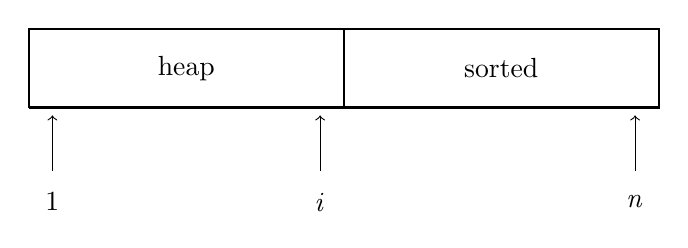
\begin{tikzpicture}
        \draw[thick] (0, 0) -- (0, 1) -- (8, 1) -- (8, 0) -- (0, 0);
	\draw[thick] (4, 0) -- (4, 1);
	\draw[->] (0.3, -0.8) -- (0.3, -0.1);
	\draw[->] (3.7, -0.8) -- (3.7, -0.1);
	\draw[->] (7.7, -0.8) -- (7.7, -0.1);
	\node at (2, 0.5) {heap};
	\node at (6, 0.5) {sorted};
	\node at (0.3, -1.2) {1};
	\node at (3.7, -1.2) {\textit{i}};
	\node at (7.7, -1.2) {\textit{n}};
    \end{tikzpicture}
\end{center}
数组中从 1 到 \textit{i} 的元素具有堆属性, 从 \textit{i}\texttt{+1} 到 
\textit{n} 是数组中最大 \textit{n}-\textit{i} 个元素, 按照升序排列.
开始时, \textit{i}=\textit{n}, 因此数组中没有已排好序的部分.

考虑上面展示的元素所组成的数组, 该数组已经具有堆属性. 在第二个阶段的第
一个步骤, 我们交换元素 \texttt{76} 和 \texttt{28}:
\begin{file}
    28 72 34 59 63 17 29 37 33 | 76
\end{file}
在第 2 个步骤, 我们把堆的大小递减到 9. 然后在第 3 个步骤中, 通过一系列的
交换操作, 把 \texttt{28} 移动到合适的位置, 从而维持住前 9 个元素的堆属性:
\begin{file}
    72 63 34 59 28 17 29 37 33 | 76
\end{file}
我们可以把这个过程可视化: 让元素 \texttt{28} 沿着二叉树的路径, 从根结点
开始, 朝着叶子结点方向, 逐渐向下渗透, 直到到达一个这样的结点: 它的孩子 
小于或等于 \texttt{28}:\footnote{TODO}

在下一次迭代中, 第一个步骤交换元素 \texttt{72} 和 \texttt{33}:
\begin{file}
    33 63 34 59 28 17 29 37 | 72 76
\end{file}
第二个步骤把 \textit{i} 递减到 8, 第三次迭代把 \texttt{33} 移动到合适的 
位置:
\marginpar{165}
\begin{file}
    63 59 34 37 28 17 29 33 | 72 76
\end{file}
下一次迭代以交换 \verb'63' 与 \verb'33' 作为开始, 迭代结束时, 序列变成:
\begin{file}
    59 37 34 33 28 17 29 | 63 72 76
\end{file}
当数组处于有序状态时, 迭代过程结束.

下面的程序对输入数据按照升序进行排列, 使用的正是上面提到的过程. 我们把 
大部分的, 由单独一条表达式组成的语句用花括号包围起来, 至于这样做的原因
将会在下一节讨论刻画时说明.
\begin{awkcode}
    # heapsort

        { A[NR] = $0 }

    END { hsort(A, NR)
          for (i = 1; i <= NR; i++)
              { print A[i] }
        }

    function hsort(A,n,  i) {
        for (i = int(n/2); i >= 1; i--)  # phase 1
             { heapify(A, i, n) }
        for (i = n; i > 1; i--) {        # phase 2
             { swap(A, 1, i) }
             { heapify(A, 1, i-1) }
        }
    }
    function heapify(A,left,right,   p,c) {
        for (p = left; (c = 2*p) <= right; p = c) {
            if (c < right && A[c+1] > A[c])
                { c++ }
            if (A[p] < A[c])
                { swap(A, c, p) }
        }
    }
    function swap(A,i,j,   t) {
        t = A[i]; A[i] = A[j]; A[j] = t
    }
\end{awkcode}

\cterm{性能}. \verb'hsort' 总的操作次数正比于 $n\log n$, 即使是在最坏的
情况下也是如此. 同样, 我们用三种类型的元素序列对 \verb'hsort' 进行性能
测试, 下面这张图显示了测试结果, 可以看到, \verb'hsort' 面对相同元素序列
时, 性能优于快速排序.\footnote{应该用矢量图}
\marginpar{166}
\begin{center}
    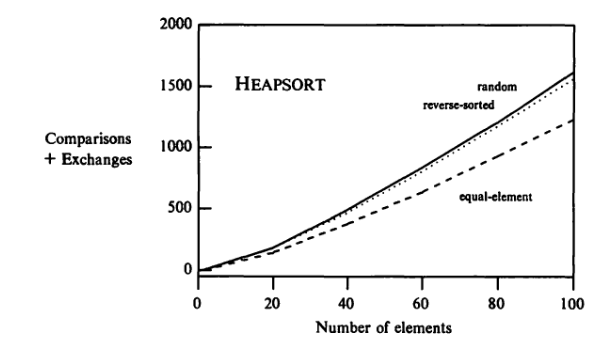
\includegraphics[scale=0.7]{images/heap_sort.png}
\end{center}

接下来的这张图显示了本节所讨论的三种排序算法, 在面对随机输入数据时的性能
表现.
\begin{center}
    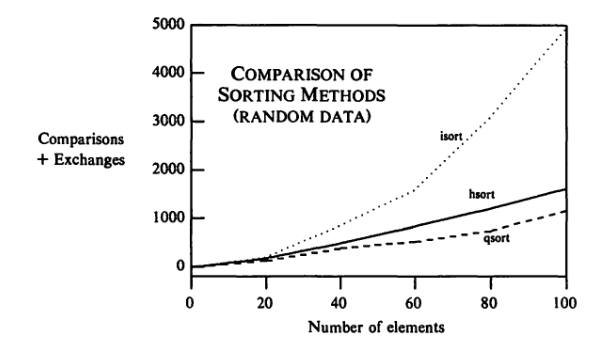
\includegraphics[scale=0.7]{images/sort_cmp.png}
\end{center}

前面曾经说过, \texttt{isort} 对随机数据进行排序的时间复杂度是二次的, 而
\texttt{hsort} 与 \texttt{qsort} 的复杂度却是 $n \log n$. 这张图清楚地
展示了一个优秀算法的重要性: 随着数据规模的增加, 二次方程序的性能与
$n \log n$ 程序性能之间的差距急剧加大.
\marginpar{167}
\begin{exercise}
    \texttt{check} 总是发现 \texttt{isort} 的输出是有序的. 对于
    \texttt{qsort} 与 \texttt{hsort} 是否也成立 ? 如果输入数据仅仅由
    数值组成, 或者是一些看起来不太像数值的字符串, 那么是否还成立 ?
\end{exercise}

% TODO "profiling" 这个词很难翻译, 我就把它译作 "剖析"
\section{剖析}
\label{sec:profiling}

在上一节中, 为了评价排序程序的性能, 我们计算了特定操作的执行次数. 评价
程序性能的另一个有效方法是对程序进行剖析, 也就是计算每条语句的执行次数.
许多编程环境都会提供一个称为 \cterm{剖析器} (\term{profiler}) 的工具
程序, 剖析器可以打印某个程序中, 每条语句的执行次数.

我们并没有为 awk 开发一个剖析器, 但是在这一节, 我们将展示如何使用两个
简短的程序, 来近似地模拟剖析器的功能. 第一个程序  \texttt{makeprof} 通过 
在代码中插入计数与打印语句, 为 awk 程序构造剖析版本. 当剖析版的程序
运行时, 它会计算每条语句的执行次数, 并把计数结果写到文件 \texttt{prof.cnts}
中. 第二个程序 \texttt{printprof} 从 \texttt{prof.cnts} 中获取语句的执行
次数, 并添加到原版程序中.

为了简单起见, 当程序运行时, 我们只对 ``可执行的'' 的左花括号进行计数.
通常来说, 这种计数安排已经足够反映问题了, 因为每一个动作, 以及每一块
组合语句都被一对花括号包围起来. 任何一条语句都可以用一对花括号包围起来,
所以, 通过为语句加花括号, 我们可以按照自己的需要来控制计数的精度.

程序 \texttt{makeprof} 把一个普通的 awk 程序转换成一个剖析版程序.
它在每个输入行的左花括号的右边插入计数语句, 计数语句具有形式:
\begin{pattern}
    \indent \texttt{\_LBcnt[}\textit{i}\texttt{]++;}
\end{pattern}
除此之外, 它还会添加一个 \verb'END' 动作, 用于输出计数结果到文件 
\texttt{prof.cnts} 中, 每行一个.
\begin{awkcode}
    # makeprof - prepare profiling version of an awk program
    #   usage:  awk -f makeprof awkprog >awkprog.p
    #   running awk -f awkprog.p data creates a
    #       file prof.cnts of statement counts for awkprog

        { if ($0 ~ /{/) sub(/{/, "{ _LBcnt[" ++_numLB "]++; ")
          print
        }

    END { printf("END { for (i = 1; i <= %d; i++)\n", _numLB)
          printf("\t\t print _LBcnt[i] > \"prof.cnts\"\n}\n")
        }
\end{awkcode}

给定一些输入数据, 运行完某个程序的剖析版之后, 我们可以用
\texttt{printprof}, 把 \texttt{protf.cnts} 中的语句计数结果附加到原始
\marginpar{168}
程序中:
\begin{awkcode}
    # printprof - print profiling counts
    #     usage:  awk -f printprof awkprog
    #     prints awkprog with statement counts from prof.cnts

    BEGIN { while (getline < "prof.cnts" > 0) cnt[++i] = $1 }
    /{/   { printf("%5d", cnt[++j]) }
          { printf("\t%s\n", $0) }
\end{awkcode}

作为示例, 考虑为 \ref{sec:sorting} 节末尾的程序 \texttt{heapsort} 作剖析.
为了构造这个程序的剖析版, 键入并执行命令
\begin{shell}
    awk -f makeprof heapsort > heapsort.p
\end{shell}
构造出的剖析版 \texttt{heapsort.p} 看起来就像:
\begin{awkcode}
    # heapsort

        { _LBcnt[1]++;  A[NR] = $0 }

    END { _LBcnt[2]++;  hsort(A, NR)
          for (i = 1; i <= NR; i++)
              { _LBcnt[3]++;  print A[i] }
        }

    function hsort(A,n,  i) { _LBcnt[4]++; 
        for (i = int(n/2); i >= 1; i--)  # phase 1
             { _LBcnt[5]++;  heapify(A, i, n) }
        for (i = n; i > 1; i--) { _LBcnt[6]++;         # phase 2
             { _LBcnt[7]++;  swap(A, 1, i) }
             { _LBcnt[8]++;  heapify(A, 1, i-1) }
        }
    }
    function heapify(A,left,right,   p,c) { _LBcnt[9]++; 
        for (p = left; (c = 2*p) <= right; p = c) { _LBcnt[10]++; 
            if (c < right && A[c+1] > A[c])
                { _LBcnt[11]++;  c++ }
            if (A[p] < A[c])
                { _LBcnt[12]++;  swap(A, c, p) }
        }
    }
    function swap(A,i,j,   t) { _LBcnt[13]++; 
        t = A[i]; A[i] = A[j]; A[j] = t
    }
    END { for (i = 1; i <= 13; i++)
                     print _LBcnt[i] > "prof.cnts"
    }
\end{awkcode}
正如你所看到的那样, 原版程序中插入了 13 条计数语句, 还额外添加了一个
\texttt{END} 动作, 该动作把计数结果输出到文件 \texttt{prof.cnts}. 多个
\texttt{END} 动作等价于按照它们出现的顺序, 组合到一个单独的 \texttt{END}
中.
\marginpar{169}

现在, 假设把 100 个随机数作为输入数据, 运行 \texttt{heapsort.p}, 程序运行 
结束后, 键入并执行命令
\begin{shell}
    awk -f printprof heapsort
\end{shell}
就可以得到带有语句执行次数的原版程序 (每条语句的执行次数仅对本次运行有效).
命令的执行结果是:
\begin{awkcode}
	# heapsort
	
  100	    { A[NR] = $0 }
	
    1	END { hsort(A, NR)
	      for (i = 1; i <= NR; i++)
  100	          { print A[i] }
	    }
	
    1	function hsort(A,n,  i) {
	    for (i = int(n/2); i >= 1; i--)  # phase 1
   50	         { heapify(A, i, n) }
   99	    for (i = n; i > 1; i--) {        # phase 2
   99	         { swap(A, 1, i) }
   99	         { heapify(A, 1, i-1) }
	    }
	}
  149	function heapify(A,left,right,   p,c) {
  526	    for (p = left; (c = 2*p) <= right; p = c) {
	        if (c < right && A[c+1] > A[c])
  228	            { c++ }
	        if (A[p] < A[c])
  473	            { swap(A, c, p) }
	    }
	}
  572	function swap(A,i,j,   t) {
	    t = A[i]; A[i] = A[j]; A[j] = t
	}
\end{awkcode}

我们实现的剖析器最重要的特点是简单, 但这同时也是它最大的缺点. 程序 
\texttt{makeprof} 盲目地在每一行的第一个左花括号的右边插入计数语句,
一个更好的做法是忽略字符串常量, 正则表达式和注释中的左花括号. 除了语句的
执行次数, 最好还要报告语句的执行时间, 但是这里介绍的方法还无法做到这
一点.

\begin{exercise}
    修改剖析器, 使得程序不会在字符串常量, 正则表达式或者注释中插入计数
    语句. 你实现的剖析器是否允许对自身进行剖析?
\end{exercise}

\begin{exercise}
    如果 \texttt{END} 动作中包含 \texttt{exit} 语句, 那么剖析器就无法
    正常地工作, 请问这是为什么 ? 修复这个问题.
\end{exercise}

\marginpar{170}
\section{拓扑排序}
\label{sec:topological_sorting}

在工程建筑项目中, 有些工作必须在其他工作开始前完成. 为了方便说明, 我们通常
会把这些工作都列出来, 这样就可以很容易地看出哪些工作必须在其他工作完成后
才能开始. 在一个程序库中, 程序 \texttt{a} 可能会调用程序 \texttt{h},
\texttt{h} 也有可能会调用程序 \texttt{d}  和 \texttt{e}, 等等. 我们可能
希望对程序进行排序, 使得程序在它调用的所有程序之前出现 (Unix 命令
\texttt{lorder} 可以完成这个工作). 这些, 以及其他类似的问题都是
\cterm{拓扑排序} (\term{topological sorting}) 问题的实例: 找到一个顺序,
该顺序满足一个约束条件集合, 集合中的每个条件都具有形式 ``\texttt{x} 必须
在 \texttt{y} 之前出现''. 由约束条件集合所表示的偏序得到该集合上的一个
线序, 这个操作叫用拓扑排序.

约束条件可以用一张图来表示, 图中的每个结点都用名字标记, 如果结点 \textit{x}
必须先于 \textit{y} 出现, 那么就有一条边, 从 \textit{x} 指向 \textit{y}.
下面这张图就是一个例子:\footnote{TODO}

如果存在一条边, 从 \textit{x} 指向 \textit{y}, 那么 \textit{x} 就是
\textit{y} 的 \cterm{前驱} (\term{predecessor}), \textit{y} 是 \textit{x}
的 \cterm{后继} (\term{successor}). 假设约束条件用 前驱-后继 对来表示,
其中每个输入行的 \textit{x} 和 \textit{y} 表示一条从结点 \textit{x} 指向 
\textit{y} 的边, 上面那张图的文本表示形式是:
\begin{file}
    a   h
    b   g
    c   f
    c   h
    d   i
    e   d
    f   b
    f   g
    h   d
    h   e
    i   b
\end{file}

如果存在一条从 \textit{x} 指向 \textit{y} 的边, 那么在输出中 \textit{x}
必须先于 \textit{y} 出现. 如果把上面的数据作为输出, 那么可能一个输出是:
\begin{file}
    a c f h e d i b g
\end{file}
除此之外, 还有其他线序关系也包含了上图所描绘的偏序, 另一个可能的线序是:
\begin{file}
    c a h e d i f b g
\end{file}

拓扑排序的目标是对图中的结点进行排序, 使得所有前驱都在它们的后继之前出现.
\marginpar{171} 当且仅当图中不含有 \cterm{环} (\term{cycle}, 是由多条边
组成的序列, 当结点沿着这个序列前进时, 最终会回到结点的原来位置) 时, 
这样的顺序才存在.

\subsection{广度优先拓扑排序}
\label{subsec:breadth_first_topological_sort}

有多种算法可以用于图的拓扑排序, 其中最简单的算法可能是 --- 在每次迭代时,
从图中移除没有前驱的结点. 如果所有的结点都按照这种方式从图中移除出来,
那么图的拓扑排序结果就是结点按照移除顺序所组成的序列. 在上面的图中, 我们 
可以从移除结点 \texttt{a} 及以它为起点的边开始, 然后移除结点 \texttt{c},
再接着是结点 \texttt{f} 或 \texttt{h}, 依此类推.

我们的实现使用了一种先进先出的数据结构 --- \cterm{队列} (\term{queue}) ---
来确定不含有前驱的结点的处理顺序, 以一种 ``广度优先'' 的方式进行.
当所有的结点都被读取完毕后, 一个循环体计算结点的数量, 并把所有的, 没有 
前驱的结点插入到队列中. 第二个循环体移除队列的第一个结点, 打印该结点的
名字, 然后递减它的每一个后继结点的前驱个数. 如果某一个后继结点的前驱
个数变为 0, 那就把这个后继结点插入到队尾. 当队列变成空, 并且所有的结点
都被访问过, 这时候拓扑排序就完成了. 但是, 如果有某些结点从未被插入到队
列中, 那就说明这些结点在一个环中, 因此无法对该图进行拓扑排序. 如果图中
不存在环, 那么被打印出来的结点序列就是一个拓扑排序.

\texttt{tsort} 的前三条语句从输入中读取 \mbox{前驱}-后继 对, 并构造一个
后继结点列表, 就像:
\begin{tabular}{c|c|c|l}
    \hline
    \hline
    \texttt{node}  & \texttt{pcnt} & \texttt{scnt} & \texttt{slist} \\
    \hline
    \texttt{a}  & 0 & 1 & \texttt{h} \\
    \texttt{b}  & 2 & 1 & \texttt{g} \\
    \texttt{c}  & 0 & 2 & \texttt{f, h} \\
    \texttt{d}  & 2 & 1 & \texttt{i} \\
    \texttt{e}  & 1 & 1 & \texttt{d} \\
    \texttt{f}  & 1 & 2 & \texttt{b, g} \\
    \texttt{g}  & 2 & 0 &  \\
    \texttt{h}  & 2 & 2 & \texttt{d, e}  \\
    \texttt{i}  & 1 & 1 & \texttt{b}  \\
    \hline
\end{tabular}

数组 \texttt{pcnt} 和 \texttt{scnt} 记录每个结点的前驱结点与后继结点个数,
\texttt{slist[}\textit{x}\texttt{,}\textit{i}\texttt{]} 给出了结点 
\textit{x} 的第 \textit{i} 个后继结点的名字. 如果 \texttt{pcnt} 中不含有
元素, 那么程序的第一行就会创建它的第一个元素.\footnote{原文为 The first
line creates an element of \texttt{pcnt} if it is not already present.}
\marginpar{172}
\begin{awkcode}
    # tsort - topological sort of a graph
    #   input:  predecessor-successor pairs
    #   output: linear order, predecessors first

        { if (!($1 in pcnt))
              pcnt[$1] = 0           # put $1 in pcnt
          pcnt[$2]++                 # count predecessors of $2
          slist[$1, ++scnt[$1]] = $2 # add $2 to successors of $1
        }
    END { for (node in pcnt) {
              nodecnt++
              if (pcnt[node] == 0)   # if it has no predecessors
                  q[++back] = node   # queue node
          }
          for (front = 1; front <= back; front++) {
              printf(" %s", node = q[front])
              for (i = 1; i <= scnt[node]; i++)
                  if (--pcnt[slist[node, i]] == 0)
                      # queue s if it has no more predecessors
                      q[++back] = slist[node, i]
          }
          if (back != nodecnt)
              print "\nerror: input contains a cycle"
          printf("\n")
        }
\end{awkcode}

在 awk 中实现队列非常简单: 只需要一个拥有两个下标的数组, 一个指向队头, 
一个指向队尾.

\begin{exercise}
    修改 \texttt{tsort}, 使得它可以处理图中孤立的结点.
\end{exercise}

\subsection{深度优先搜索}
\label{subsec:depth_first_search}

为了说明深度优先搜索技术, 我们将再构造一个拓扑排序程序. 深度优先搜索可以
用来解决与图相关的许多问题, 包括 Unix 实用程序 \texttt{make} 中蕴含的图
问题. 深度优先搜索是另一种遍历图结点的系统化方法, 即使是在含有环的图中.
在最简单的形式中, 深度优先搜索只是一个递归过程:
\begin{pattern}
    \indent dfs(\textit{node}): \par
    \indent\indent mark \textit{node} visited
    \indent\indent for all unvisited successors \textit{s} of \textit{node}
                do \par
    \indent\indent\indent dfs(\textit{s})
\end{pattern}
之所以称为 ``深度优先'' 是因为搜索从一个结点开始, 然后访问该结点的某个
未被访问过的后继结点, 再接着访问该后继结点的某个未被访问过的后继结点,
依此类推, 基本原则是尽可能快地向图的纵向深入. 如果某个结点的所有后继
结点都被访问过了, 搜索过程就回退到前驱结点, 然后再按照深度优先的方法,
搜索前驱结点的另一个未被访问过的后继结点.

\marginpar{173}
考虑下面的这张图. 如果遍历从结点 1 开始, 那么深度优先搜索将会陆续访问
结点 1, 2, 3 和 4. 这时候, 如果从另一个未访问过的结点开始, 比如 5, 那么 
接下来将会访问结点 5, 6 和 7. 如果遍历从不同的结点开始, 那么将会得到不同
的结点访问序列.\footnote{TODO}

深度优先搜索可以用来判断图中是否含有环. 如果有一条边指向的是之前访问过
的祖先结点, 比如 \texttt{(3, 1)}, 那么这条边就叫作\cterm{回边} (\term{back
edge}). 因为存在回边等同于存在环, 所以为了判断图中是否含有环, 我们只 
需要搜索回边就够了. 下面的函数判断某个图是否存在结点 \texttt{node} 
可到达的环, 图用后继结点列表来表示, 这个数据结构我们已经在 \texttt{tsort}
中见过.
\begin{awkcode}
    # dfs - depth-first search for cycles

    function dfs(node,     i, s) {
        visited[node] = 1
        for (i = 1; i <= scnt[node]; i++)
            if (visited[s = slist[node, i]] == 0)
                dfs(s)
            else if (visited[s] == 1)
                print "cycle with back edge (" node ", " s ")" 
        visited[node] = 2
    }
\end{awkcode}

这个函数使用数组 \texttt{visited} 来判断某个结点是否被访问过. 开始时,
\texttt{visited[}\textit{x}\texttt{]} 等于 0. 在第一次进入结点 \textit{x}
时, \texttt{dfs} 把 \texttt{visited[}\textit{x}\texttt{]} 设置为 1,
最后一次离开结点 \textit{x} 时, 把 \texttt{visited[}\textit{x}\texttt{]}
设置为 2. 在遍历过程中, \texttt{dfs} 利用 \texttt{visited} 来判断结点
\textit{y} 是否是当前结点的祖先 (以及它之前是否被访问过). 如果 \textit{y}
是当前结点的祖先, 那么 \texttt{visited[}\textit{y}\texttt{]} 等于 1,
如果 \textit{y} 之前被访问过, 那么 \texttt{visited[}\textit{y}\texttt{]} 
的值就等于 1.\footnote{TODO 需要仔细检查这段话 --- 译者注}

\subsection{深度优先拓扑排序}
\label{subsec:depth_first_topological_sort}

函数 \texttt{dfs} 很容易就可以修改为结点排序例程. 一旦从某结点开始的
搜索过程结束, 如果在此时打印该结点的名字, 那么所打印出来的结点序列刚好就
是逆序的拓扑排序, 前提是图中不含有环. 给定一个 \mbox{前驱}-后续\ 对序列
作为输入数据, 程序 \texttt{rtsort} 输出图的逆序拓扑排序, 它对每一个
没有前驱的结点应用深度优先搜索. 程序中使用的数据结构与 \texttt{tsort}
中的相同.
\marginpar{174}
\begin{awkcode}
    # rtsort - reverse topological sort
    #   input:  predecessor-successor pairs
    #   output: linear order, successors first

        { if (!($1 in pcnt))
              pcnt[$1] = 0           # put $1 in pcnt
          pcnt[$2]++                 # count predecessors of $2
          slist[$1, ++scnt[$1]] = $2 # add $2 to successors of $1
        }

    END { for (node in pcnt) {
              nodecnt++
              if (pcnt[node] == 0)
                  rtsort(node)
          }
          if (pncnt != nodecnt)
              print "error: input contains a cycle"
          printf("\n")
        }

    function rtsort(node,     i, s) {
        visited[node] = 1
        for (i = 1; i <= scnt[node]; i++)
            if (visited[s = slist[node, i]] == 0)
                rtsort(s)
            else if (visited[s] == 1)
                printf("error: nodes %s and %s are in a cycle\n",
                    s, node)
        visited[node] = 2
        printf(" %s", node)
        pncnt++    # count nodes printed
    }
\end{awkcode}

如果把本节开头给出的 \mbox{前驱}-后继 对作为输入数据, 这个程序将会输出:
\begin{shell}
    g b i d e h a f c
\end{shell}
需要注意的是, 对图中的某些环来说, 这个程序可以通过查找回边来显式地探测,
而对另一些环的探测则是隐式地, 对于后一种情况, 程序将无法打印出全部的结点,
就像这幅图:\footnote{TODO}


\begin{exercise}
    修改 \texttt{rtsort}, 按照通常的顺序打印结点, 也就是先打印前驱结点.
    你是否可以在不修改 \texttt{rtsort} 的前提下达到同样的效果?
\end{exercise}

\marginpar{175}
\section{Make: 文件更新程序}
\label{sec:make_a_file_updating_program}

大型程序中包含的声明与子例程通常分布在多个文件中, 通过一系列复杂的处理
步骤来生成最终的程序. 一篇复杂的文档 (比如本章) 可能由许多图表和程序组成,
这些图表和程序代码存放在不同的文件中, 而且程序会被运行和测试, 最终将通过
一系列互相依赖的操作来生成可打印的文档. 如果有一个自动更新工具能够在
消耗最小的人力物力的前提下, 完成这些处理工作, 那么这个工具的价值将是无法
衡量的. 本节将仿照 Unix 命令 \texttt{make}, 开发一个具备基本功能的
更新程序, 基本算法是上节讨论过的深度优先搜索.

为了使用更新程序, 用户必须显式地描述出系统的组成成分, 各个成分之间的依
赖关系, 以及构造它们的命令. 我们假设依赖关系和构造命令存放在一个文件中, 
文件名是 \texttt{makefile}, 里面包含了一系列规则, 每条规则都具有形式:
\begin{pattern}
    \indent\textit{name}:\texttt{    }$t_1$\ $t_2$\ ...\ $t_n$ \par 
    \indent\indent\textit{command}
\end{pattern}
规则的第一行是依赖关系, 意思是程序或文件 \textit{name} 依赖于目标
$t_1$, $t_2$, ..., $t_n$, 其中 $t_i$ 是文件名或另一个 \textit{name}.
依赖关系的下面是一行或多行 \textit{command}, 这些 \textit{command} 是
用来生成 \textit{name} 的的命令. 下面显示的是某个小程序的
\texttt{makefile} 文件, 程序由两个 C 文件和一个 \texttt{yacc} 语法文件
组成 (\texttt{yacc} 是一个典型的用于程序开发的应用程序):
\begin{file}
    prog:       a.o b.o c.o
                cc a.o b.o c.o -ly -o prog 
    a.o:        prog.h a.c
                cc -c prog.h a.c
    b.o:        prog.h b.c
                cc -c prog.h b.c
    c.o:        c.c
                cc -c c.c
    c.c:        c.y
                yacc c.y
                mv y.tab.c c.c
    print:
                pr prog.h a.c b.c c.y
\end{file}
第1行表示 \texttt{prog} 依赖于目标文件 \texttt{a.o}, \texttt{b.o} 和
\texttt{c.o}. 第2行是说使用 C 编译器 \texttt{cc} 链接 \texttt{a.o},
\texttt{b.o}, \texttt{c.o} 和一个库文件来生成 \texttt{prog}. 下一条规则
(第3行) 表示 \texttt{a.o} 依赖于目标 \texttt{prog.h} 和 \texttt{a.c},
通过编译这 2 个文件来生成 \texttt{a.o}, \texttt{b.o} 是类似的. 文件 
\texttt{c.o} 依赖于 \texttt{c.c}, 而后者依赖于 \texttt{c.y}, \texttt{c.y}
将会被 \texttt{yacc} 处理. 最后, 名字 \texttt{print} 不依赖于任何目标,
按照惯例, 对于没有目标的名字, \texttt{make} 总是会执行后面的命令,
在这里是用命令 \texttt{pr} 打印所有的源代码文件.

\marginpar{176}
\texttt{makefile} 中的依赖关系可以用一张图来表示, 如果依赖性规则左边的
\textit{x} 依赖于右边的目标 \textit{y}, 那么在图中就有一条边从结点
\textit{x} 指向 结点 \textit{y}. 如果某条规则没有目标, 就在图中创建一
个没有后继的结点, 并用规则左边的名字来命令. 上文的 \texttt{makefile}
对应的依赖图是:\footnote{TODO}

如果在 \textit{x} 的最后一次修改之后, \textit{y} 才会被修改, 那么, 我们 
就认为 \textit{x} 比 \textit{y} \cterm{老} (\term{older}). 为了跟踪年龄,
对每一个 \textit{x} 都有一个对应的整数 \texttt{age[}\textit{x}\texttt{]},
后者表示自从 \textit{x} 上一次被修改之后, 已经过了多长时间. 年龄值越大,
说明文件越老: 如果 \texttt{age[}\textit{x}\texttt{]} $\geqslant$ 
\texttt{age[}\textit{y}\texttt{]}, 则 \textit{x} 比 \textit{y} 老.

如果存在一条依赖关系:
\begin{shell}
    n: a b c
\end{shell}
那么在更新 \texttt{n} 之前, 需要先更新 \texttt{a},\texttt{b} 和 \texttt{c},
而在更新后面 3 个时, 也需要按照依赖关系来进行. 如果 \texttt{makefile}
中的某个目标既不是一个名字, 也不是某个已存在的文件, 程序就报错并退出.
否则的话, 检查目标的年龄, 如果至少有一个目标的年龄比 \texttt{n} 的年龄
小 (也就是说, \texttt{n} 比某些依赖还老), 我们就执行依赖关系下面的命令.
命令执行完毕后, 重新计算所有对象的年龄. 如果有一条规则是:
\begin{shell}
    print:
                pr prog.h a.c b.c c.y
\end{shell}
这是一条没有目标的规则, 对于这些规则, 我们总是执行和该规则相关的命令,
并更新对象的年龄.

程序 \texttt{make} 接收一个 \texttt{name} 作为输入参数, 并采用下面的
算法来更新 \textit{name}:
\begin{enumerate}
    \item 
        在 \texttt{makefile} 中搜索 \textit{name} 对应的规则, 并递归
        地更新依赖关系右边的目标 $t_1$, $t_2$, ..., $t_n$, 如果某个 
        $t_i$ 不是一个名字, 或者文件 $t_i$ 不存在, 程序就会中止更新过程.
    \item 
        在更新完所有的 $t_i$ 之后, 如果当前的 \textit{name} 比某个
        $t_i$ 老, 又或者是 \texttt{name} 没有目标, 程序就会执行依赖
        关系下面的命令.
\end{enumerate}
\marginpar{177}

在本质上, 本节所使用的方法和上一节的方法是一样的, \texttt{make} 根据
\texttt{makefile} 中的依赖关系来构造依赖图, 它使用 Unix 命令 
\begin{shell}
    ls -t
\end{shell}
对文件进行排序 (越新的文件越靠前), 排序的依据是文件最后的修改时间. 文件 
名将作为数组 \texttt{age} 的索引, 而数组元素的值则是文件在排序序列中的
名次, 最老的文件拥有最大值的名次. 如果规则中的名字不是当前目录中的文件
名, \texttt{make} 就把它的时间设置成一个很大的值.

最后, \texttt{make} 使用上一节讲过的深度优先搜索来遍历依赖图. 在节点
\textit{n}, \texttt{make} 遍历 \textit{n} 的后继节点, 如果存在某个后继
节点, 它的年龄比 \textit{n} 的年龄小, \texttt{make} 就执行规则中的命令,
并计算出一套新的年龄. 如果 \texttt{make} 发现某个名字的依赖关系存在环,
程序就会报错并中止更新过程.

为了说明 \texttt{make} 如何工作, 假设我们现在是第一次键入并执行命令
\begin{shell}
    make prog
\end{shell}
\texttt{make} 将会执行以下命令序列:
\begin{shell}
    cc -c prog.h a.c
    cc -c prog.h b.c
    yacc c.y
    mv y.tab.c c.c
    cc -c c.c
    cc a.o b.o c.o -ly -o prog
\end{shell}
如果我们对 \texttt{b.c} 作了修改, 然后再次键入
\begin{shell}
    make prog
\end{shell}
\texttt{make} 只会执行
\begin{shell}
    cc -c prog.h b.c
    cc a.o b.o c.o -ly -o prog
\end{shell}
因为在上一次创建 \texttt{prog} 之后, 其他文件并没有被修改过, 所以 
\texttt{make} 并不会对它们进行处理. 最后, 如果我们再次执行
\begin{shell}
    make prog
\end{shell}
\texttt{make} 将会输出
\begin{shell}
    prog is up to date
\end{shell}
因为文件没有发生变化, 所以什么也不需要做.
\marginpar{178}
\begin{awkcode}
    # make - maintain dependencies

    BEGIN {
        while (getline <"makefile" > 0)
            if ($0 ~ /^[A-Za-z]/) {  #  $1: $2 $3 ...
                sub(/:/, "")
                if (++names[nm = $1] > 1)
                    error(nm " is multiply defined")
                for (i = 2; i <= NF; i++) # remember targets
                    slist[nm, ++scnt[nm]] = $i
            } else if ($0 ~ /^\t/)        # remember cmd for
                cmd[nm] = cmd[nm] $0 "\n" #   current name
            else if (NF > 0)
                error("illegal line in makefile: " $0)
        ages()      # compute initial ages
        if (ARGV[1] in names) {
            if (update(ARGV[1]) == 0)
                print ARGV[1] " is up to date"
        } else
            error(ARGV[1] " is not in makefile")
    }

    function ages(      f,n,t) {
        for (t = 1; ("ls -t" | getline f) > 0; t++)
            age[f] = t   # all existing files get an age
        close("ls -t")
        for (n in names)
            if (!(n in age))   # if n has not been created
                age[n] = 9999  # make n really old
    }
    function update(n,   changed,i,s) {
        if (!(n in age)) error(n " does not exist")
        if (!(n in names)) return 0
        changed = 0
        visited[n] = 1
        for (i = 1; i <= scnt[n]; i++) {
            if (visited[s = slist[n, i]] == 0) update(s)
            else if (visited[s] == 1)
                error(s " and " n " are circularly defined")
            if (age[s] <= age[n]) changed++
        }
        visited[n] = 2
        if (changed || scnt[n] == 0) {
            printf("%s", cmd[n])
            system(cmd[n])  # execute cmd associated with n
            ages()          # recompute all ages
            age[n] = 0      # make n very new
            return 1
        }
        return 0
    }
    function error(s) { print "error: " s; exit }
\end{awkcode}

\marginpar{179}
\begin{exercise}
    在示例中, 函数 \texttt{ages} 会执行多少次?
\end{exercise}

\begin{exercise}
    添加一些参数或宏替换功能, 使得我们可以很容易地对规则进行修改.
\end{exercise}

\begin{exercise}
    为常见的更新操作添加隐式规则, 例如, 使用 \texttt{cc} 编译 
    \texttt{.c} 文件来生成 \texttt{.o} 文件. 你将会用什么方法来表示
    隐式规则, 使得用户可以对这些规则进行修改?
\end{exercise}
